\begin{frame}
  \begin{enumerate}
    \item
      Use the interactive decision procedure to check if object is invariant
      confluent.
    \pause\item
      If it is, deploy it with weak consistency.
    \pause\item
      If it's not, then...? \pause deploy with strong consistency?
  \end{enumerate}

  \note{%
    With our decision procedure in hand, here's how we deploy a distributed
    object. First, we use the decision procdure to check if the object is
    invariant confluent. If it is, then we deploy it with weak consistency
    knowing its invariant will be maintained. If it's not, then we'll what can
    we do? I mean, we can deploy the object with strong consistency, but it
    seems like overkill.
  }
\end{frame}

\newcommand{\dy}{0.2}
\begin{frame}
  \begin{center}
    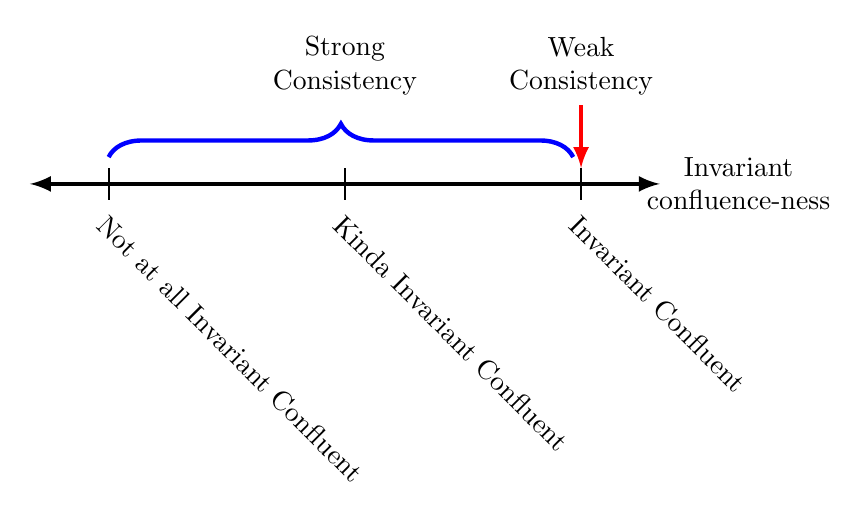
\begin{tikzpicture}
      \draw[ultra thick, latex-latex] (0, 0) to (8, 0);
      \draw[thick] (1, -\dy) to (1, \dy);
      \draw[thick] (4, -\dy) to (4, \dy);
      \draw[thick] (7, -\dy) to (7, \dy);
      \node[align=center] at (9, 0) {Invariant\\confluence-ness};
      \pause
      \node[rotate=-45, anchor=north west] at (7, -\dy) {Invariant Confluent};
      \pause
      \node[rotate=-45, anchor=north west] at (4, -\dy) {Kinda Invariant Confluent};
      \pause
      \node[rotate=-45, anchor=north west] at (1, -\dy) {Not at all Invariant Confluent};

      \pause
      \draw[ultra thick, -latex, red] (7, 1) to (7, \dy);
      \node[align=center, fill=white] at (7, 1.5) {Weak\\Consistency};

      \pause
      \draw[decorate, decoration={brace, amplitude=12pt, raise=4pt},
            ultra thick, blue] (1, \dy) to (6.9, \dy);
      \node[align=center] at (4, 1.5) {Strong\\Consistency};
    \end{tikzpicture}
  \end{center}

  \note{%
    If we think about it long enough, we'll realize that invariant
    confluence-ness is actually a spectrum. We have fully invariant confluent
    objects like, our bank account example with deposits. We have kinda
    invariant conluent objects, like our bank account with deposits and
    withdrawals. And we have objects that are not at all invariant confluent,
    like our bank account with only withdrawals.

    If our object is completely invariant confluent, then we can deploy it with
    weak consistency. But if it's even just a smidge not invariant confluent,
    then we're forced to use strong consistency.
  }
\end{frame}

\begin{frame}
  \begin{center}
    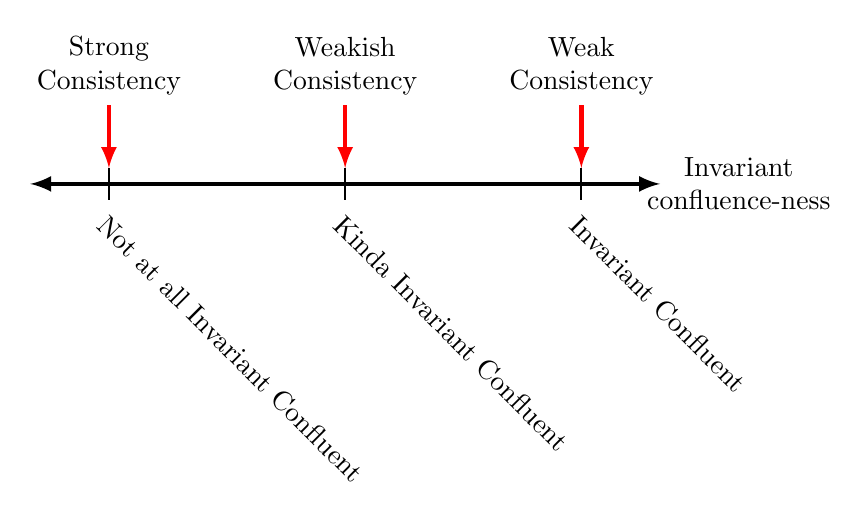
\begin{tikzpicture}
      \draw[ultra thick, latex-latex] (0, 0) to (8, 0);
      \draw[thick] (1, -\dy) to (1, \dy);
      \draw[thick] (4, -\dy) to (4, \dy);
      \draw[thick] (7, -\dy) to (7, \dy);
      \node[align=center] at (9, 0) {Invariant\\confluence-ness};
      \node[rotate=-45, anchor=north west] at (7, -\dy) {Invariant Confluent};
      \node[rotate=-45, anchor=north west] at (4, -\dy) {Kinda Invariant Confluent};
      \node[rotate=-45, anchor=north west] at (1, -\dy) {Not at all Invariant Confluent};

      \draw[ultra thick, -latex, red] (7, 1) to (7, \dy);
      \node[align=center, fill=white] at (7, 1.5) {Weak\\Consistency};
      \draw[ultra thick, -latex, red] (4, 1) to (4, \dy);
      \node[align=center, fill=white] at (4, 1.5) {Weakish\\Consistency};
      \draw[ultra thick, -latex, red] (1, 1) to (1, \dy);
      \node[align=center, fill=white] at (1, 1.5) {Strong\\Consistency};
    \end{tikzpicture}
  \end{center}

  \note{%
    This is not ideal.  Ideally, we would have a spectrum of coordination to
    match our spectrum of invariant confluence-ness.  Invariant confluent
    objects could use weak consistency. Objects that are kinda invariant
    confluent could use weakish consistency. And, objects that are not at all
    invariant confluent could use strong consistency.
  }
\end{frame}

\begin{frame}
  \begin{center}
    \Large
    \defword{Segmented invariant confluence}: divide state space into segments;
    operate with weak consistency within segments and strong consistency across
    segments.
  \end{center}

  \note{%
    Well, we can accomplish such a thing using a technique called segmented
    invariant confluence. I don't have time to go into the details, but the
    main idea is to divide the state space into segments.
  }
\end{frame}

\tikzstyle{point}=[shape=circle, fill=flatgray, inner sep=2pt, draw=black]
\tikzstyle{region}=[draw=none]
\tikzstyle{region1}=[region, fill=flatred!50]
\tikzstyle{region2}=[region, fill=flatgreen!50]
\tikzstyle{region3}=[region, fill=flatblue!50]
\tikzstyle{region4}=[region, fill=flatpurple!50]

\newcommand{\pointgrid}[4]{{
  \newcommand{\argxmin}{#1}
  \newcommand{\argxmax}{#2}
  \newcommand{\argymin}{#3}
  \newcommand{\argymax}{#4}

  \draw[] (\argxmin, 0) to (\argxmax, 0);
  \draw[] (0, \argymin) to (0, \argymax);
  \foreach \x in {\argxmin, ..., \argxmax} {
    \foreach \y in {\argymin, ..., \argymax} {
      \node[point] (\x-\y) at (\x, \y) {};
    }
  }
}}

\newcommand{\subfigwidth}{0.24\columnwidth}
\newcommand{\subfighspace}{0.3cm}
\newcommand{\tikzhspace}{0.4cm}
\newcommand{\tikzscale}{0.75}
\newcommand{\xmin}{-2}
\newcommand{\xmax}{2}
\newcommand{\ymin}{-2}
\newcommand{\ymax}{2}

\begin{frame}
  \begin{center}
    \begin{tikzpicture}[scale=\tikzscale]
      \draw[white] (-3, -3) to (3, 3);
      \draw[region1] (\xmin.5, \ymax.5) rectangle (-0.5, 0.5);
      \draw (-0.5, 0.5) to (\xmin.5, 0.5);
      \draw (-0.5, 0.5) to (-0.5, \ymax.5);
      \pointgrid{\xmin}{\xmax}{\ymin}{\ymax}
    \end{tikzpicture}%
    \hspace{0.1in}%
    \begin{tikzpicture}[scale=\tikzscale]
      \draw[white] (-3, -3) to (3, 3);
      \draw[region2] (-0.5, 0.5) rectangle (\xmax.5, \ymin.5);
      \draw (-0.5, 0.5) to (\xmax.5, 0.5);
      \draw (-0.5, 0.5) to (-0.5, \ymin.5);
      \pointgrid{\xmin}{\xmax}{\ymin}{\ymax}
    \end{tikzpicture}

    \begin{tikzpicture}[scale=\tikzscale]
      \draw[white] (-3, -3) to (3, 3);
      \draw[region3] (-0.5, \ymax.5) rectangle (0.5, \ymin.5);
      \draw (-0.5, \ymax.5) to (-0.5, \ymin.5);
      \draw (0.5, \ymax.5) to (0.5, \ymin.5);
      \pointgrid{\xmin}{\xmax}{\ymin}{\ymax}
    \end{tikzpicture}%
    \hspace{0.1in}%
    \begin{tikzpicture}[scale=\tikzscale]
      \draw[white] (-3, -3) to (3, 3);
      \draw[region4] (\xmin.5, 0.5) rectangle (\xmax.5, -0.5);
      \draw (\xmax.5, -0.5) to (\xmin.5, -0.5);
      \draw (\xmax.5, 0.5) to (\xmin.5, 0.5);
      \pointgrid{\xmin}{\xmax}{\ymin}{\ymax}
    \end{tikzpicture}
  \end{center}

  \note{%
    Returning to our example from before, we can divide our state space into
    the second quadrant, the fourth quadrant, the y-axis and the x-axis.
    \\[12pt]

    Within each segment, replicas can operate without coordination, but when
    transitioning across segment boundaries, replicas have to coordinate.
    \\[12pt]

    In our paper, we formalize segmented invariant confluence, explain how to
    deploy segmented invariant confluent objects, and develop another decision
    procedure for segmented invariant confluence. If you're interested in those
    details, I encourage you to check out our paper. \\[12pt]
  }
\end{frame}

\begin{frame}
  A segmentation $\Sigma = (I_1, T_1), \ldots, (I_n, T_n)$ is a sequence (not a
  set) of $n$ segments $(I_i, T_i)$ where every $T_i$ is a subset of $T$ and
  every $I_i \subseteq S$ is an invariant.
\end{frame}

\begin{frame}
  \begin{algorithmic}
    \If{$t \notin T_i$}
      \State Execute $t$ with global coordination
    \Else{}
      \If{$I_i(t(s_i))$} Commit $t$
      \ElsIf{$\lnot I(t(s_i))$} Abort $t$
      \Else{} Execute $t$ with global coordination
      \EndIf{}
    \EndIf{}
  \end{algorithmic}
\end{frame}
